\section{Simulink model}
Before we can implement the control system, what we have created for the cube, on the microcontroller we must simulate it.
For the simulation we have designed a nonlinear and linear controller in simulink.

The highest level of the system will be shown on the figure below.
\begin{figure}[H]

	
	\centering
 	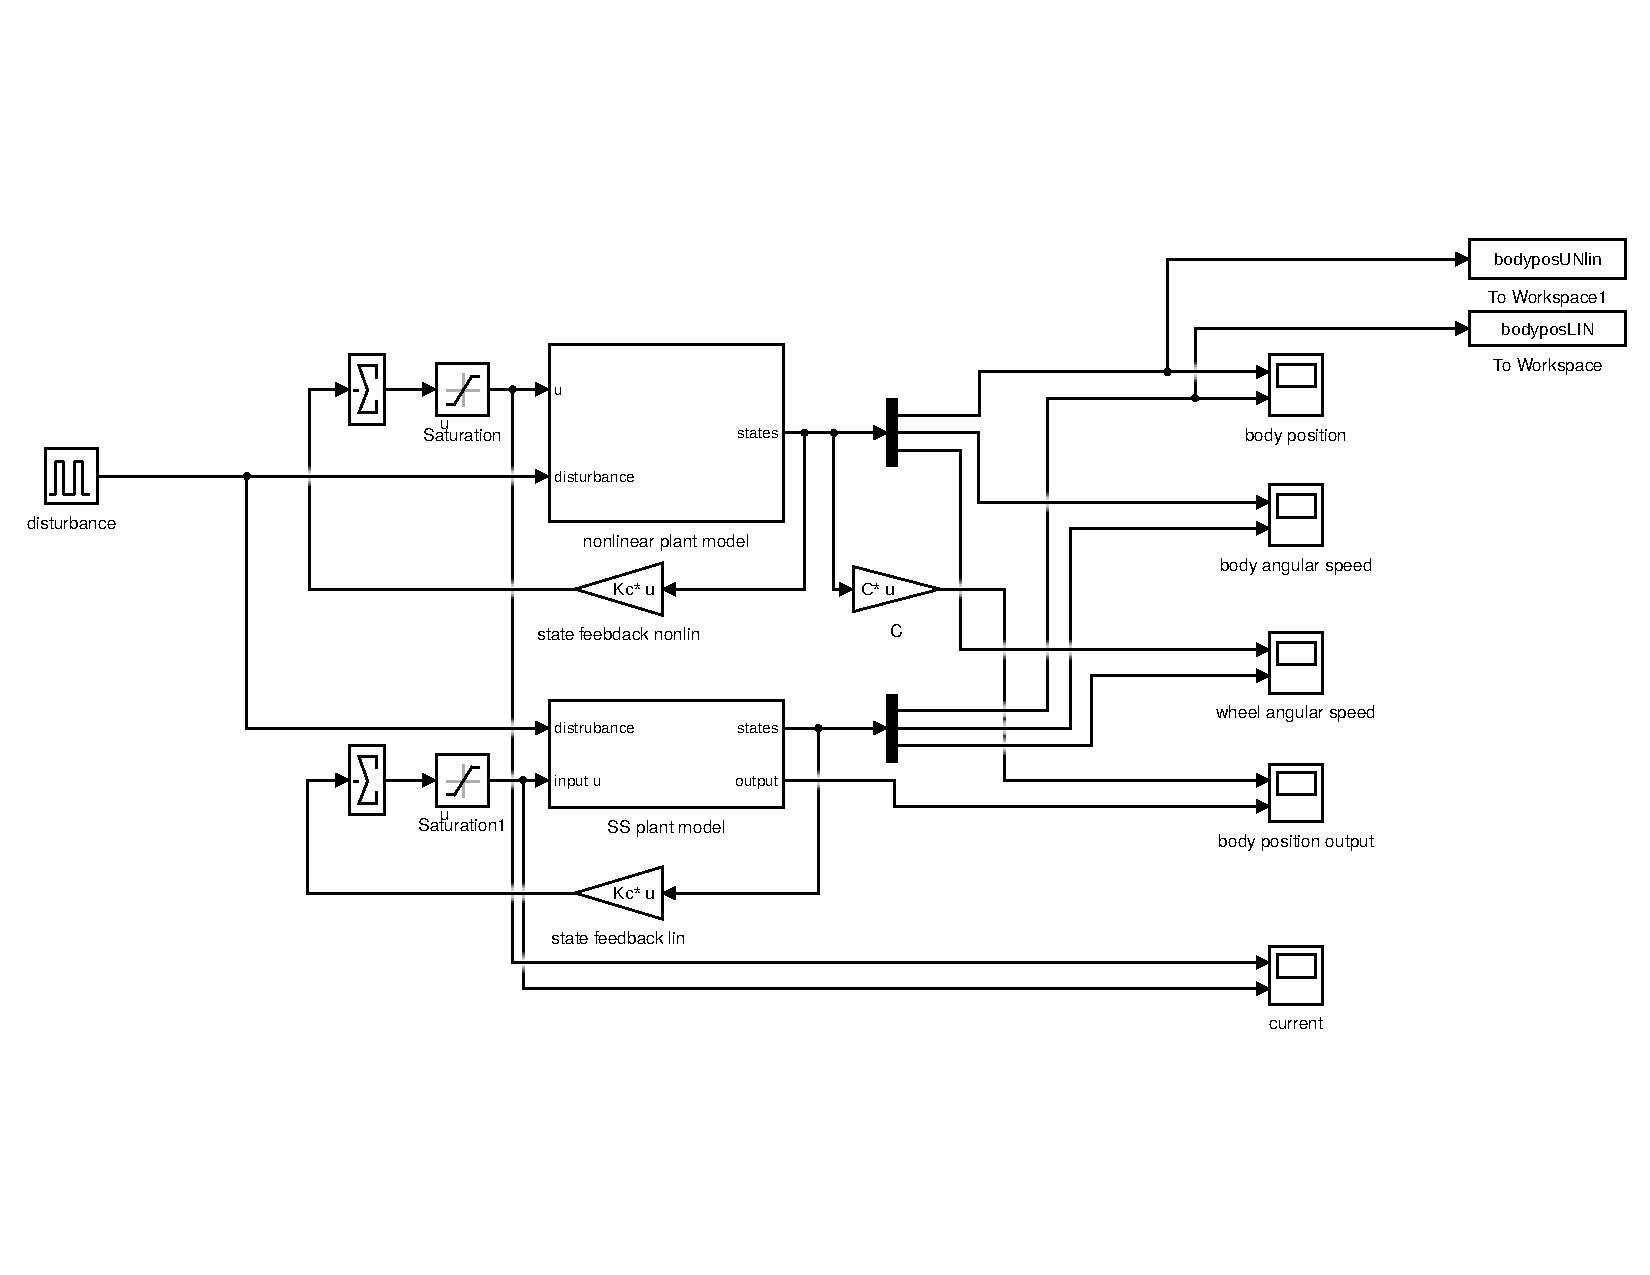
\includegraphics[width=1\textwidth]{images/systemmodel.pdf}
	
	~
	\caption{Highest level of the system} 
 	\label{fig:mech} 
\end{figure}

Here we can see the two systems what we created the top loop named nonlinear plant model is the nonlinear state space model of the system.
The bottom loop what is named SS plant model what is the linear model of the system.
The linearization was made by using the small angle approximation principle where $sin(x)=x$ \cite{smallangle}.

\clearpage
In the following figure we can see the nonlinear plant model upclose.
\begin{figure}[H]

	
	\centering
 	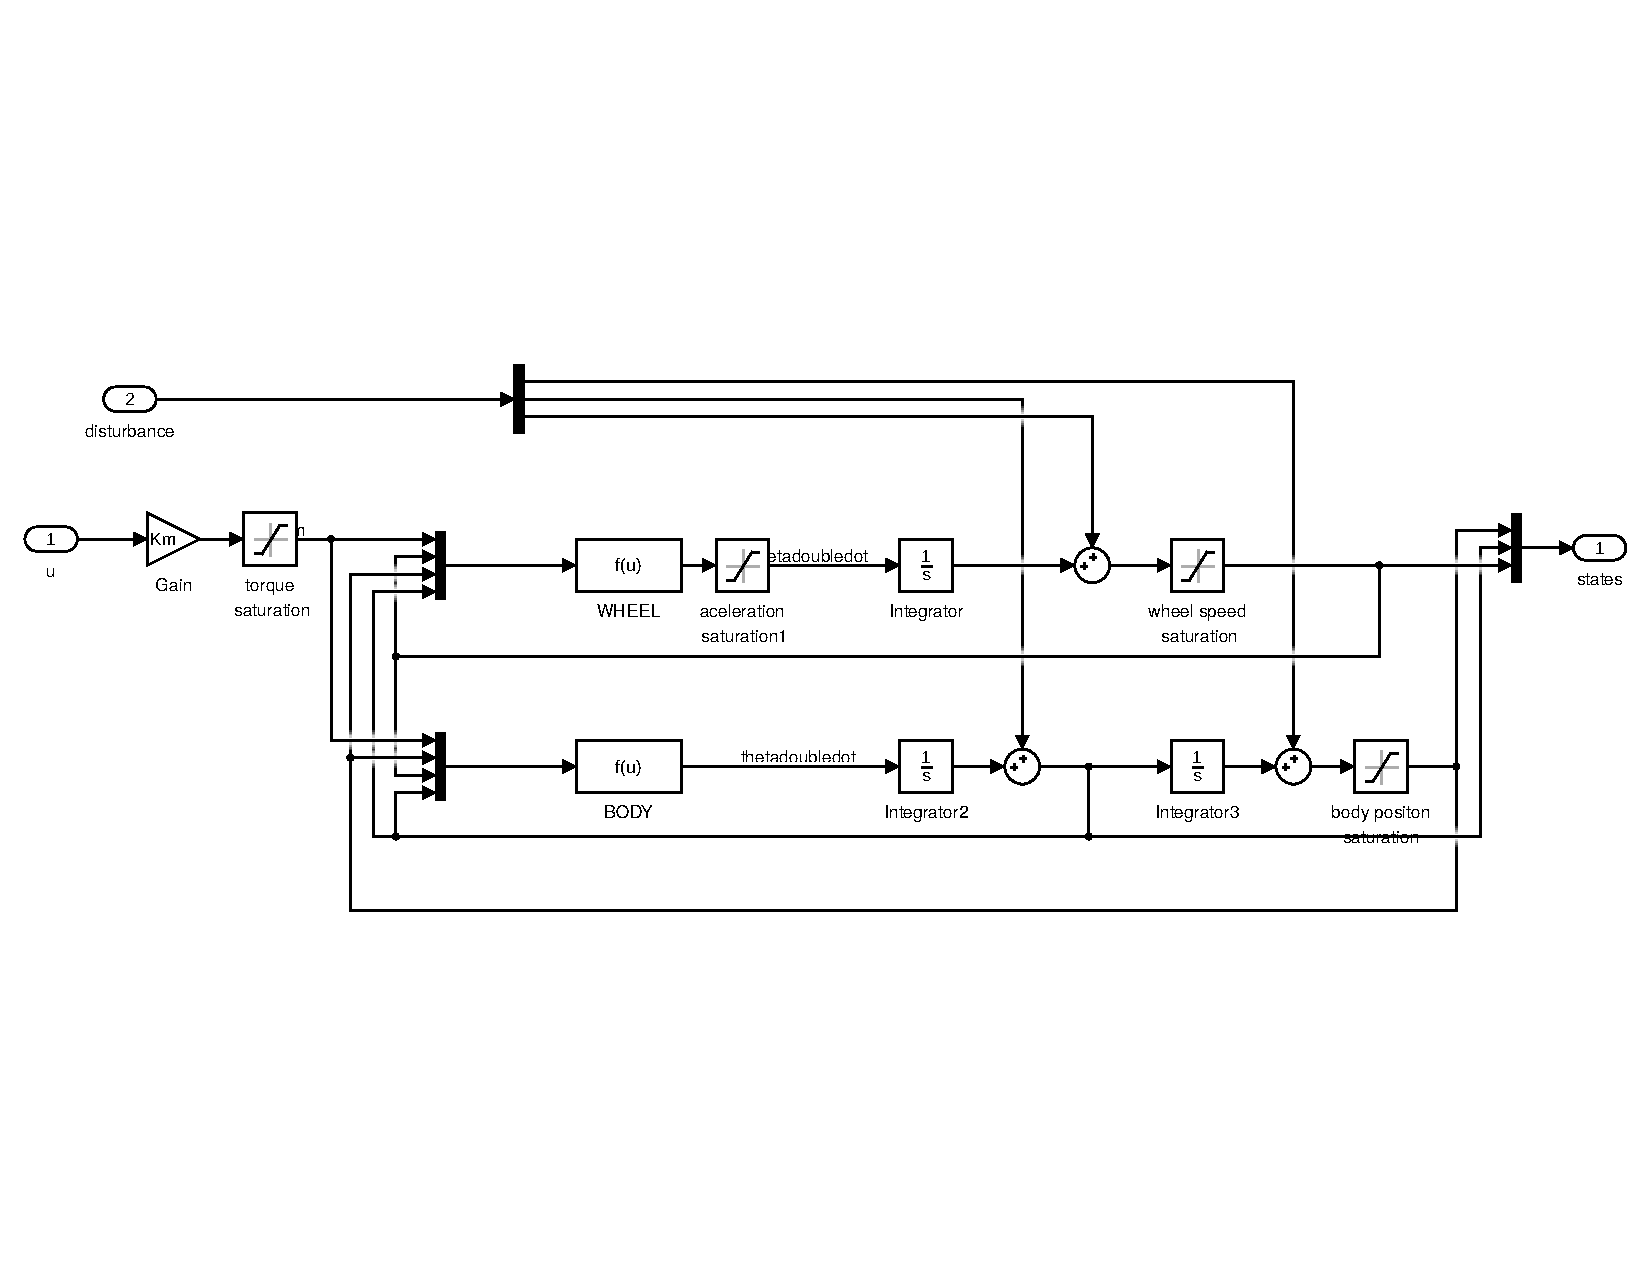
\includegraphics[width=1\textwidth]{images/nonlin.pdf}
	
	~
	\caption{Nonlinear plant model} 
 	\label{fig:mech} 
\end{figure}

\clearpage
Following figure below shows the linear plant model where we used the small angle approximation.
\begin{figure}[H]

	
	\centering
 	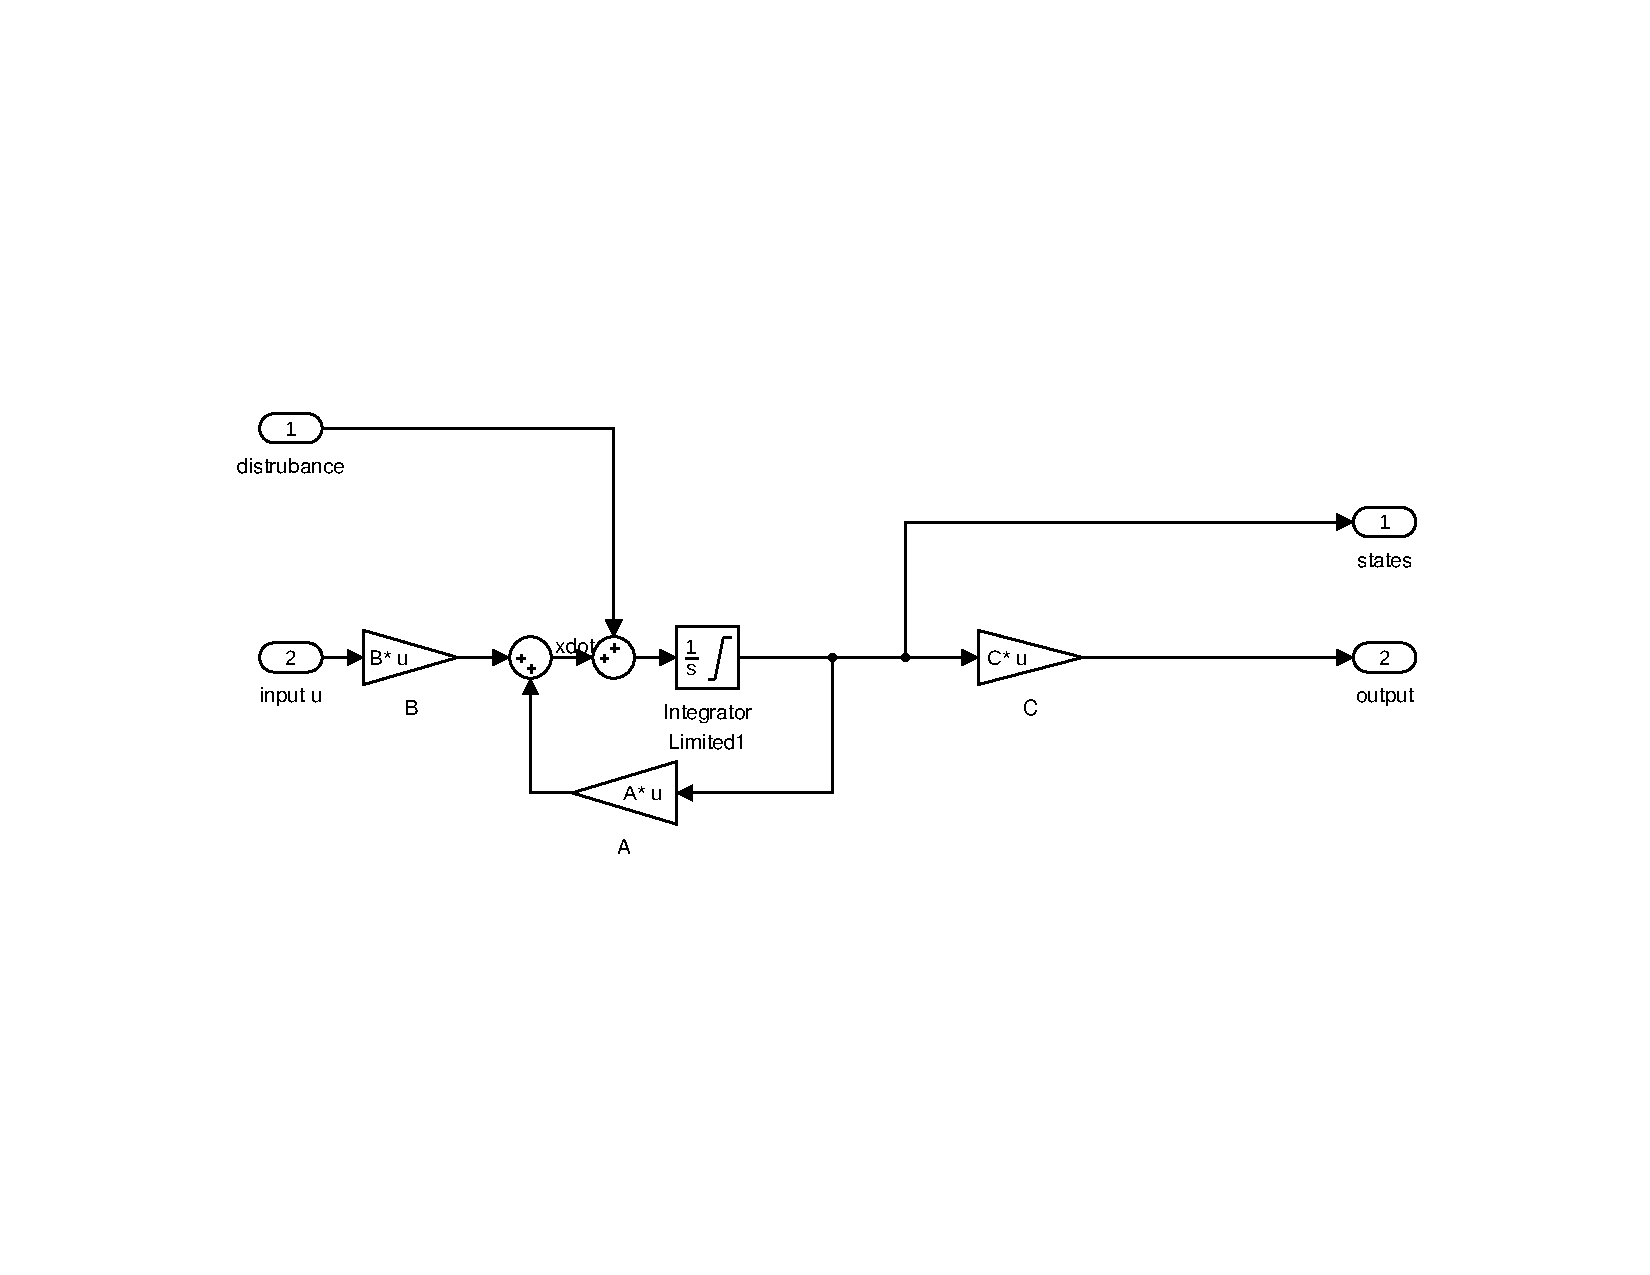
\includegraphics[width=1\textwidth]{images/ssnon.pdf}
	
	~
	\caption{Linear plant model} 
 	\label{fig:mech} 
\end{figure}

As it is shown on all the models we are using the saturations to evaluate the maximal values of the inputs and outputs according to our set parameters.
On the body position we have the max values of 1,6rad and -1,6rad what are approximately 90 degrees and -90 degrees.
These both are the positions where the cube is on one or the other side.
The current saturation has the maximum and minimum values 5 and -5 ampers what are the maximum currents that the motor is taking.
In the wheel speed saturation we have the maximum values of the wheel speed what are give on the datasheet.
Maximum and minimum wheel speeds are in our case 628rad/s and -628rad/s.
In the torque saturation are the maximum and minimum values of the maximum constant torque that the motor can supply.
According to the datasheet they are 0,0834 Nm and - 0,0834 Nm.

On all the following graphs the yellow line shows the nonlinear model and the blue line is the linear model.

We ran a simulation with a disturbance of 0,4rad and 0,1s and we got the following results:
\begin{figure}[H]

	
	\centering
 	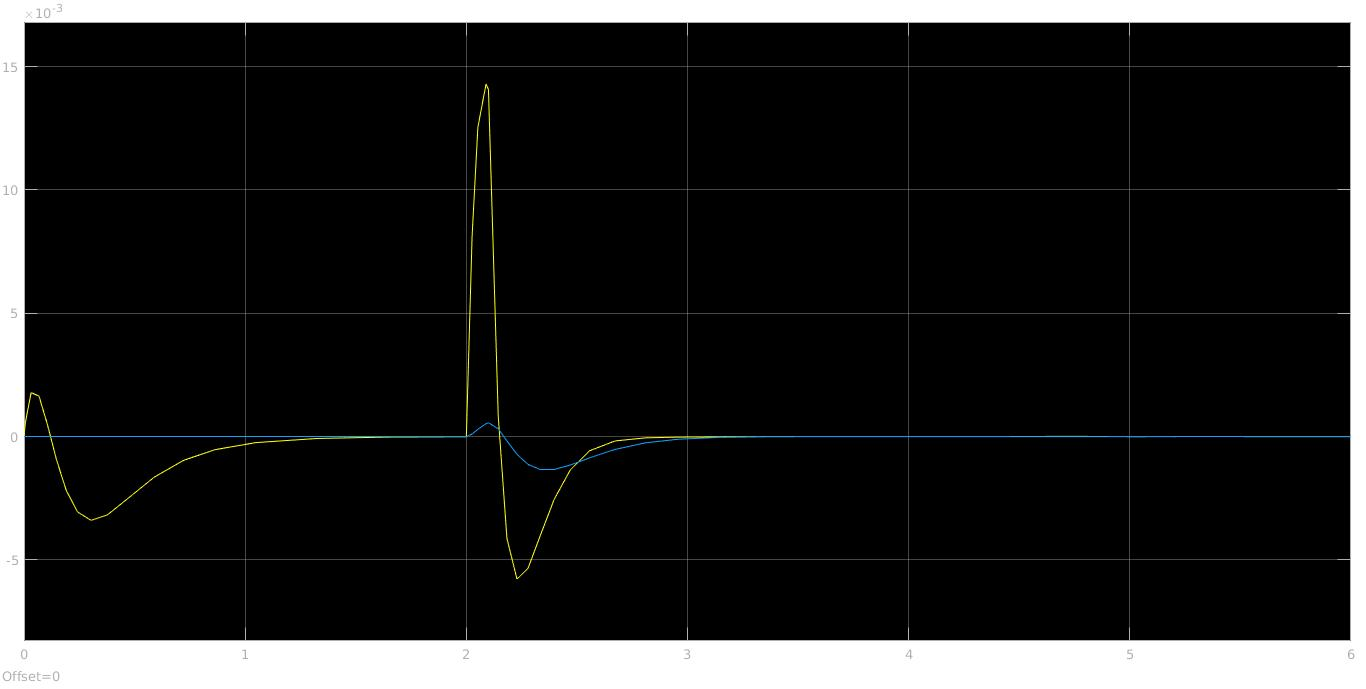
\includegraphics[width=1\textwidth]{images/pos0401.jpg}
	
	~
	\caption{Body position while balancing} 
 	\label{fig:mech} 
\end{figure}

Following graph shows the bodys angular speed during the simulation.
\begin{figure}[H]

	
	\centering
 	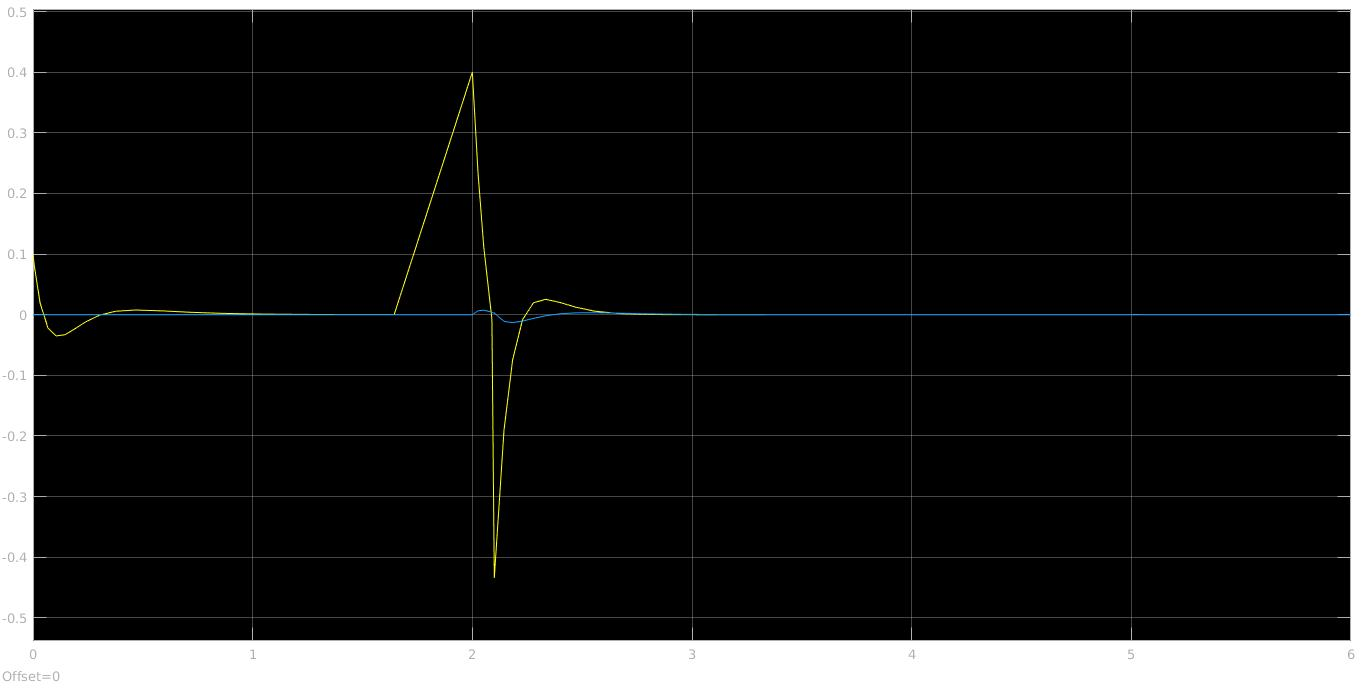
\includegraphics[width=1\textwidth]{images/acc0401.jpg}
	
	~
	\caption{Body speed while balancing} 
 	\label{fig:mech} 
\end{figure}

Next one is the current input to the motor.
\begin{figure}[H]

	
	\centering
 	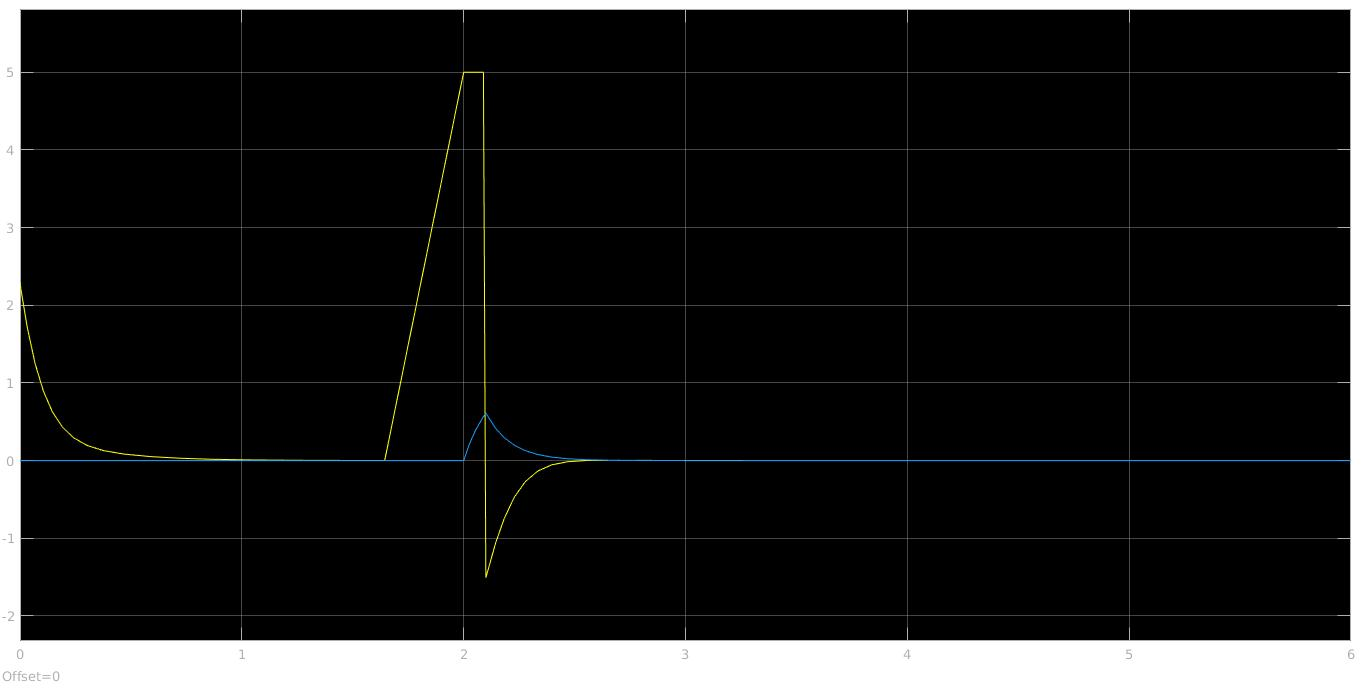
\includegraphics[width=1\textwidth]{images/curr0401.jpg}
	
	~
	\caption{Current input while balancing} 
 	\label{fig:mech} 
\end{figure}

And the final graph is the angular speed of the reaction wheel.
\begin{figure}[H]

	
	\centering
 	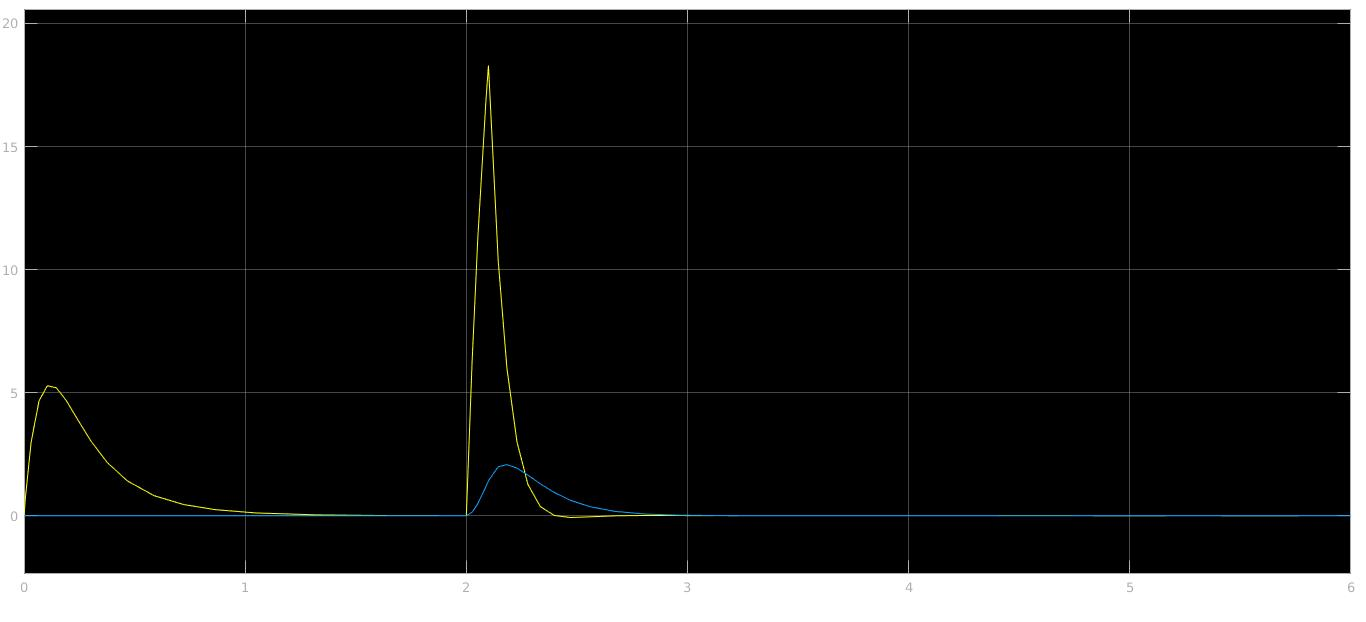
\includegraphics[width=1\textwidth]{images/wspeed0401.jpg}
	
	~
	\caption{Reaction wheel angular speed while balancing} 
 	\label{fig:mech} 
\end{figure}

While simulating the balancing we tested through different amplitudes and found that the maximum disturbance that the system can balance is approximately 22 degrees.
From that we can say that our system is stable and able to balance itself up to 22 degrees offset from the balanceing point.
If the angle is bigger then the 22 degrees the system will tilt over because the motor is not strong enough to counteract the earths gravity.

